\chapter{Hashmap Algorithms and Analysis}
\label{hashmap}

This chapter investigates different concurrent and transactional algorithms for hashmaps. We begin with an overview of concurrent and transactional hashmap specifications and algorithms. We then evaluate how these hashmaps perform on several microbenchmarks, and discuss why and how particular highly-concurrent hashmap algorithms, modified to provide transactional guarantees, can outperform our current transactional algorithms.

\section{Algorithms}

We present the concurrent and transactional algorithms we analyzed, created, and implemented in our work. Some general terminology: an \emph{element} refers to the key-value pair inserted into the hashmap. A \emph{bucket} is a container of elements, and a hashmap consists of a set of buckets. The algorithms differ in the methods used to place elements in buckets and track how buckets and elements are modified.

\subsection{Transactional Chaining Hashmap}
The STO chaining hashmap (ChainingHashmap) is a concurrent, transactional hashmap implemented using a standard chaining algorithm. If two elements are mapped to the same bucket, they are chained in a linked list. Thus, the worst case lookup/delete is $O(n)$. Inserts are always constant time and require allocating an element. Each bucket is associated with a \emph{bucketversion} that increments upon any committed addition or removal from the bucket. The bucketversion is used to verify that no thread has added an element that was absent during a transaction's find. In addition, each bucket has a lock that synchronizes access to the bucket. Each inserted element is associated with an \emph{elementversion} that tracks if the value to the element has been modified or if the element has been removed.

Elements are inserted at execution time but marked as \emph{phantom}, allowing another transaction that sees ones of these uninstalled elements to realize it is viewing an inconsistent state of the map and therefore abort. If a transaction containing insertions aborts, these phantom elements are removed from the map. ELse thephantom mark is erased during commit. An alternative approach would be to insert all elements at commit time.However, this requires either relying on the bucketversion to determine if another transaction has inserted the same element (which would result in false aborts since the bucketversion increments for \emph{any} inserted value) or redoing the search for the element to see if the insertion can still occur. Thus, we insert at execution time to allow for more fine-grained validation checks at commit time and to reduce redundant computations. Deletions are delayed until commit time (an optimistic approach). This requires careful handling of cases of \emph{read\_my\_writes}, such as deleting an element inserted in the same transaction, 

\subsection{Non-Transactional Cuckoo Hashmap}
The Non-Transactional Cuckoo Hashmap (CuckooNT) implements a concurrent, non-transactional cuckoo hashing algorithm (implementation modified from \cite{cuckoocode}).

Each element is placed in one of two buckets; these buckets are determined by two different hash functions. A bucket has a fixed size of elements. This means that lookups and deletes only require executing two hash functions and checking the contents of two buckets (an $O(1)$ operation).

Inserts run in amortized time $O(1)$ but may occasionally be $O(n)$.
If an element $e$ is hashed by the first hash function to a bucket that is already full, the algorithm attempts to place $e$ in its alternative bucket by hashing $e$ with the second hash function. If both buckets are full, cuckoo shuffling occurs. This process kicks out an element $e'$ in one of $e$'s buckets and places $e'$ in $e'$'s alternative bucket. If $e'$'s alternative bucket is full, an element $e''$ is ejected from this bucket, and so on. As long as the cuckoo shuffling does not encounter a bucket cycle, $e$ can now be placed in one of its buckets, as the removal of $e'$ has made space for $e$.
However, if the shuffling encounters a bucket cycle, the hashmap raises an \texttt{out of space} assertion error. We can imagine an alternative implementation that allows the hashmap to grow in number of buckets or otherwise change its hash functions, reinserting all elements, but for simplicity, we keep the algorithm statically sized.

Because the buckets are statically sized, elements are contained in fixed-size key and value arrays and therefore do not require extra allocations.

\subsection{Transactional Cuckoo Hashmap}
The transactional cuckoo hashmap comes in three flavors: allocating, allocating with key-fragments, and non-allocating. All flavors instrument the non-transactional cuckoo hashmap with STO calls that provide transactional guarantees.
Both allocating and non-allocating versions use the same synchronization algorithm: like the STO chaining hashmap, each bucket has a \emph{bucketversion} and lock and each element has an \emph{elementversion}. Because insertions can occur due to cuckoo shuffling as well as an external insertion call, the bucketversion increments only when an element \emph{not already contained in the map} is inserted into the bucket (i.e., elements inserted via a call to insert and not via cuckoo shuffling). Elements are inserted at execution time with a \emph{phantom} flag that is then erased at commit time, and deletions are delayed until commit time.

The allocating transactional cuckoo hashmaps allocate elements upon insertion. One variant (CuckooIE) contains buckets containing pointers to the elements, allowing STO to track elements by their memory address to verify elementversions at commit time. The key-fragments variant (CuckooKF) expands buckets to contain both an array of keys and an array of element pointers. This enables a lookup or delete for an absent item to skip following the pointer to the allocated internal element itself, and can reduce the number of cache line accesses depending on the workload.

The non-allocating transactional cuckoo hashmap consists of buckets consisting of a fixed-sized array of wrapped elements. STO tracks elements by their keys. Therefore, to verify if an elementversion has changed at commit time, the check procedure performs a find of the element using the key (searching at most two buckets) and validates the corresponding elementversion. Although this reduces the number of allocations, elementversions can now move between buckets, and the values in their previous locations invalidated. This complicates correctly checking and synchronizing the reads of elementversions.

\section{Evaluation}

\subsection{Microbenchmarks}
As with the queue, all hashmaps queues are evaluated on a set of microbenchmarks to demonstrate their scalability and performance. The controlled nature of these microbenchmarks allow us to easily compare particular aspects of each algorithm, such as transactional overhead introduced by STO. All experiments are run on the same machine as the queue experiments (with 100GB DRAM, two 6-core Intel Xeon X5690 processors with hyperthreading clocked at 3.47GHz and a 64-bit Linux 3.2.0 operating system). All benchmarks and STO data structures are compiled with \texttt{g++-5.3}. In all graphs, we show the median of 5 consecutive runs with the minimum and maximum performance results represented as error bars.

\subsubsection{Parameters}

\begin{itemize}
    \item Proportion of Finds/Inserts/Deletes: The ratio of inserts:deletes is kept at 1 to ensure that the hashmap does not always become empty or only grow in size. It is expected that half the inserts will succeed and half the deletes will succeed, since both are drawing key values from the same range. Tests of 5\% inserts, 5\% deletes, and 90\% finds simulate the most likely use cases for hashmaps\cite{hm1}. Tests of equal proportion (33\%) of all operations investigate how the hashmap reacts to an increased rate of inserts and deletes.
    \item Operations per transaction: We choose to run all tests comparing transactional to non-transactional (parallel-only) data structures using single-operation transactions. As discussed in Section~\ref{q_microbenchmarks}, this provides a more fair evaluation of transactional data structures against concurrent ones. In addition, it allows us to minimize the differences between transaction hashmap implementations so we can get a baseline comparison.
    \item Number of buckets: Both the cuckoo hashmaps and the chaining hashmap statically set the number of buckets in the data structure. The number of elements allowed in one bucket of the cuckoo hashmaps is fixed at a particular value, which we will call the \emph{maximum fullness}. 
        The \emph{capacity} (number of buckets $\times$ number of elements per bucket) of the cuckoo hashmap is fixed at some finite value because the cuckoo hashmap has a fixed size bucket; the chaining hashmap has no fixed capacity because a bucket's chain can grow arbitrarily long.
        The number of buckets and the size of each bucket affects the number of cache lines accessed during the test (for example, a larger hashmap may not be expected to fit into the L2 cache, whereas a small hashmap at full capacity will fit entirely in cache). During all tests, the number of keys present in the hashmap is not allowed to outgrow its capacity.
    \item Fullness: The ratio equivalent to (number of keys : number of buckets). This determines the average number of elements to be found per bucket. The tests are implemented such that at steady state, fullness is expected to be 75\% of the maximum fullness of the cuckoo hashmap to avoid an out-of-space exception. This is controlled by picking a maximum key value. The maximum key value of inserted elements is twice the number of elements the hashmap will contain when its size reaches a fixed point.
\end{itemize}
Note that the initial size of the data structure should not affect performance as the test proceeds for a longer period of time and reaches a steady state. Therefore, we do not include the initial size as a benchmark parameter.

\subsubsection{Multi-Thread, Variable-Capacity Singletons Test} 
This test is run with different numbers of threads and with different proportions of finds/inserts/deletes. Each thread runs 5 million singleton transactions.
The test is run twice, once with a probability of 33\% insert, 33\% delete, and 34\% find, and again with a probability of 5\% insert, 5\% delete, and 90\% find. The steady-state final size is 50\% maximum load.

\subsection{Results and Discussion}

We measure all hashmap's performance in terms of operations per second, abort rates, and cache performance (number of cache misses). 
The full results can be found in Appendix~\ref{app:hashmaps}.

\subsubsection{Hypothesis 1: The transactional cuckoo hashmaps will experience a greater number of cache misses}

    \begin{figure}[t]
    \centering
        \begin{minipage}{0.45\textwidth}
        \centering
        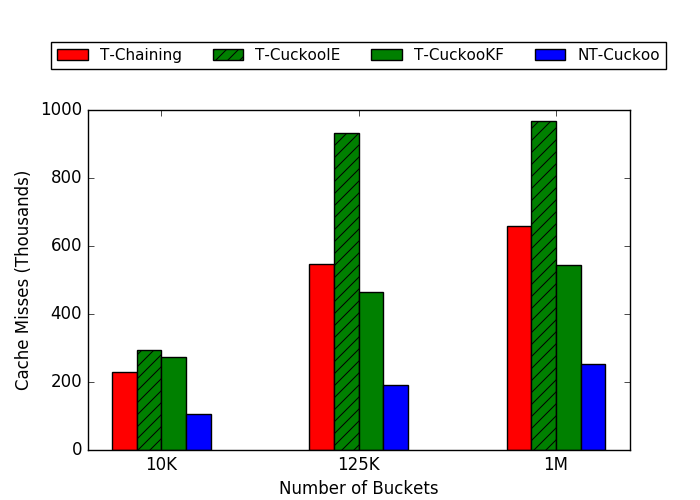
\includegraphics[width=\textwidth]{maps/3310cm.png}
        \caption*{33\%Find, 33\%Insert, 33\% Delete}
        \end{minipage}
        \begin{minipage}{0.45\textwidth}
            \centering
            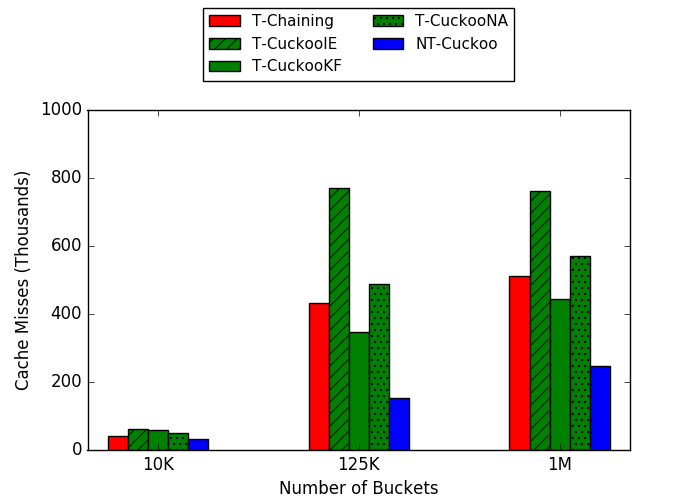
\includegraphics[width=\textwidth]{maps/9010cm.png}
            \caption*{90\%Find, 5\%Insert, 5\% Delete}
        \end{minipage}
        \caption{Hashmap Cache Misses (Max Fullness 10)}
    \end{figure}


The number of cache misses of each datatype is influenced by the number of allocations per data structure and the patterns in which these allocations are accessed. As expected, the non-transactional cuckoo hashmap experiences the least number of cache misses: this is because all other hashmaps' buckets contain a pointer to an allocated element inserted into the map. We expect that the non-allocating, transactional cuckoo hashmap will perform better than either of the allocating types \lyt{TODO?}.

Overall, the CuckooIE hashmap experiences the most cache misses as a result of both the cuckoo hashing algorithm: two buckets and all pointers to elements within the buckets are accessed during a find. As size and fullness increases, the CuckooKF hashmap experiences the least number of cache misses: this likely occurs because a find will not need to follow pointers in a CuckooKF hashmap bucket to compare key values, whereas comparing key values in the chaining and CuckooIE hashmaps both require following pointers.

\subsubsection{Hypothesis 2: Increases in the number of buckets and maximum fullness of the hahmap increases the number of cache misses by about the same amount in all hashmaps}

As expected, maps of size 10K buckets experience the fewest cache misses regardless of the maximum fullness allowed: this is because the table and all its elements fit entirely in cache. There is no significant difference in the number of cache misses between hashmaps of size 125K and 1M buckets for either the 33\% Finds/Inserts/Erases  or 90\% Finds, 5\% Inserts/Erases Test. This may be attributed to the greater probability of short chains / empty buckets during the time before the hashmap reaches a fixed point in the number of keys the map contains: since the number of threads running the tests is fixed at 8 threads, the number of keys in the map reaches this fixed point more slowly with 1M buckets than with 125K buckets.

As maximum fullness increases from 5 to 10, all transactional hashmaps experience an increase in the number of cache misses. Both the chaining and cuckoo hashmaps will iterate on average through more elements per bucket during a find, therefore increasing the number of cache misses. The chaining and CuckooIE hashmaps experience a greater increase from a maximum fullness of 10 to 15 than does the CuckooKF hashmap; this is likely due to the optimizations taken for key comparison in the CuckooKF hashmap.

\subsubsection{Hypothesis 3: The abort rate decreases as the number of buckets increases, but performance is not heavily affected by abort rate}

    \begin{table}[t]
    \centering
        \begin{minipage}{0.45\textwidth}
        \centering
        \begin{tabular}{|c|c|c|c|}
\hline
\multirow{2}{*}{Hashmap} & \multicolumn{3}{c|}{\#Threads Abort Rate (\%)}\\\cline{2-4}& 4 & 12 & 20\\
\hline
\hline
T-Chaining & 0.003 & 0.013 & 0.021\\
T-CuckooIE & 0.001 & 0.004 & 0.005\\
T-CuckooKF & 0.001 & 0.004 & 0.007\\
NT-Cuckoo & 0.000 & 0.000 & 0.000\\
\hline
\end{tabular}

        \caption*{10K Buckets}
        \end{minipage}
        \begin{minipage}{0.45\textwidth}
        \centering
        \begin{tabular}{|c|c|c|c|}
\hline
\multirow{2}{*}{Hashmap} & \multicolumn{3}{c|}{\#Threads}\\\cline{2-4}& 4 & 12 & 20\\
\hline
\hline
T-Chaining & 0.000 & 0.002 & 0.002\\
T-CuckooIE & 0.000 & 0.000 & 0.001\\
T-CuckooKF & 0.000 & 0.000 & 0.001\\
NT-Cuckoo & 0.000 & 0.000 & 0.000\\
\hline
\end{tabular}

        \caption*{125K Buckets}
        \end{minipage}
        \begin{minipage}{0.45\textwidth}
        \centering
        \begin{tabular}{|c|c|c|c|}
\hline
\multirow{2}{*}{Hashmap} & \multicolumn{3}{c|}{\#Threads}\\\cline{2-4}& 4 & 12 & 20\\
\hline
\hline
T-Chaining & 0.00004 & 0.34599 & 0.13496\\
T-CuckooA & 0.00001 & 0.15493 & 0.04467\\
T-CuckooKF & 0.00001 & 0.09270 & 0.06208\\
NT-Cuckoo & 0.00000 & 0.00000 & 0.00000\\
\hline
\end{tabular}

        \caption*{1 Million Buckets}
        \end{minipage}
        \caption{Hashmap Abort Rate (Max Fullness 10, 33\%F/33\%I/33\%E)}
    \end{table}

Overall, the abort rate remains relatively constant regardless of the fullness of the hashmap, but decreases as the number of buckets in the map increases. A greater number of buckets decreases the abort rates, since the probability that two threads will simultaneously attempt to read/modify the same bucket decreases. Abort rate is negligible in nearly all tests, with the chaining hashmap experiencing the highest abort rates (the median of 5 trials never exceeding 0.006\%)

We see that cache performance affects overall performance more than the abort rate: as the number of buckets and thus the number of cache misses increases, the performance decreases even though abort rate also decreases.

\subsubsection{Hypothesis 4: The behaviors of the transactional cuckoo hashmap and the transactional chaining hashmap do not differ the behaviors of their nontransactional counterparts. }

In the 90\% Finds, 5\% Inserts/Erases Test, the performance of the cuckoo hashmaps decreases by approximately 33\% as hashmap size increases from 10K to 1M buckets. However, the chaining hashmap experiences nearly no decrease in performance, or at times, an increase in performance to nearly 150\% its original performance. The CuckooKF hashmap at 10K buckets achieves performance $2\times$ that of the chaining hashmap. Performance is approximately equivalent for all transactional hashmaps at 125K buckets, and at 1M buckets the chaining hashmap achieves performance up to $1.5\times$ that of the cuckoo hashmaps. These performance differences are exacerbated as the fullness of the maps grows. This is expected since increased fullness results in a more significant increase in the numbers of cache misses in the cuckoo hashmaps.
 Performance on this test is nearly $1.5\times$ that of the 33\% Finds/Inserts/Erases Test. This is expected, since a find is both faster to perform than an insert or delete, and a find requires only reading a bucketversion for all transactional hashmaps.

In the 33\% Finds/Inserts/Erases Test, the performance of the cuckoo hashmaps decreases only slightly (less than 20\%) as hashmap size increases from 10K to 1M buckets. However, the chaining hashmap experiences nearly no decrease in performance. For all fullness settings, the cuckoo hashmaps achieve performance approximately $1.5-2\times$ that of the chaining hashmap for when the size is set to 10K or 125K buckets. Performance is approximately equivalent when the size is set to 1M buckets.

We note that the behavior of the transactional cuckoo hashmap mirrors that of the nontransactional cuckoo hashmap, although the performance is of the transactional version is consistently about half that of the nontransactional. Our expectations for how the cuckoo hashing algorithm performs compared to a chaining algorithm are consistent to the results we see when we compare the transactional cuckoo hashmap to the transactional chaining hashmap.
More specifically, the transactional cuckoo hashmap outperforms the chaining hashmap when run on a large maximum fullness with a small number of buckets. 

Thus, unlike the flat combining queue, the cuckoo hashmap does not experience crippling performance loss when integrated into a transactional setting. This is because the cuckoo hashmap algorithm's optimizations pertain even in the transactional setting: the speedup of the cuckoo hashmap algorithm results from the constant time lookups and deletes, and amortized constant time insertions. These asymptotic time bounds still apply to our transactional algorithms for cuckoo hashmap operations.

Furthermore, the overhead incurred by adding transactional guarantees to the cuckoo hashmap is no more than the overhead incurred by adding the same guarantees to the chaining hashmap. A transactional find in a cuckoo hashmap and a chaining hashmap adds to the read set an object representing the bucket in which the object should be (or is) located.  A transactional insert requires adding a read (and write, depending if the inserted key is already present) of the bucket in which the object should be located. A transactional erase requires adding a read (and write, depending if the key to erase is present) of the bucket the object should be located. Thus, the granularity of conflicts is still per-bucket, and the core optimizations which the cuckoo hashmap takes to achieve better performance than the chaining hashmap in particular scenarios are still applicable. In other words, the modifications required to provide transactional guarantees and the characteristics of cuckoo hashing that provide its performance benefits are orthogonal.
